\section{Financial Markets as Self-Computing Systems: Complete Theory}

This section presents the complete theoretical foundation \cite{kotikov2025}, demonstrating how financial markets serve as natural examples of self-computing functorial objects and providing the deeper mathematical context for Natural Observation-Based Computing.

\subsection{Markets as Symbolic Sequences}

\subsubsection{From Empirical Data to Symbolic DNA}

Financial market data ($OHLCV$: Open, High, Low, Close, Volume) represents an empirical projection of deeper symbolic dynamics. Historical data can be transformed into symbols ($S$ --- Supply, $D$ --- Demand, $N$ --- Neutral, $R$ --- Reversal, $T$ --- Trend, etc.) based on relative changes and correlations.

The temporal market series becomes a string:
\begin{equation}
\sigma_{\text{market}} = SDDNRTTSP\ldots \in \Sigma^*
\end{equation}

This is the \textbf{empirical symbolic DNA} of the market. In the symbolic structures framework \cite{kotikov2025}, we fix the mapping:
\begin{equation}
F_{\text{mkt}}: \Sigma^* \to \Sigma^*
\end{equation}
which transforms the previous market state (symbol string) into the next state at each step.

\subsubsection{Meta-Levels of Self-Computing in Markets}

\begin{table}[h]
\centering
\small
\begin{tabular}{@{}cp{4.5cm}p{5cm}@{}}
\toprule
\textbf{Depth} & \textbf{System Representation} & \textbf{Economic Analogue} \\ \midrule
0 & Simple trend dynamics (``IF trend THEN continue'') & Classical AR/MA models \\
1 & Agent reacts to market (feedback loop) & Technical trading \\
2 & Agent changes strategy in response to other agents' dynamics & Adaptive algorithms, high-frequency trading \\
3 & Agents mutually model each others' models & Game dynamics, Nash invariants \\
4 & Meta-system includes observer (market knows it's being watched) & Self-fulfilling expectations \\
5 & Self-reflexive layer (emotions, narratives, politics) & Macroeconomic memory of market \\ \bottomrule
\end{tabular}
\caption{Meta-levels of self-computation in financial markets}
\label{tab:market_metalevels}
\end{table}

\subsection{Predictability Limits in Markets}

Markets have no pure stochasticity --- what appears random is \textbf{inaccessibility of symbolic structure}: we don't know the complete symbolic ``genome'' (all hidden meta-levels of reflection).

Therefore, predictability $\Psi(d)$ can be interpreted as:
\begin{itemize}
    \item For $d \leq 1$: system nearly deterministic, linear models apply
    \item For $1 < d < 3$: partially predictable through patterns, suitable for symbolic analysis (pattern matching)
    \item For $d \geq 3$: self-modifying structure emerges: any prediction attempt becomes \emph{part of the system} (feedback interference)
\end{itemize}

\subsection{Depth Metric for Markets}

To estimate self-computing depth $d_{\text{mkt}}$, we construct three observable indicators:

\begin{enumerate}
    \item \textbf{Information Reflexivity:} Correlation between market reaction and participant expectations
    
    \item \textbf{Symbolic Sequence Entropy:} Diversity of pattern formations --- higher entropy indicates more hidden levels:
    \begin{equation}
    H(\sigma) = -\sum_{i} p_i \log p_i
    \end{equation}
    where $p_i$ is frequency of pattern $i$
    
    \item \textbf{Algorithm Learning Speed:} Rate of change in market strategy dynamics
\end{enumerate}

Empirically, $d_{\text{mkt}} \approx 3\ldots 4$: the system predicts its own predictions.

\subsection{Computational Models for Markets}

\begin{table}[h]
\centering
\begin{tabular}{@{}p{4cm}p{4cm}p{5cm}@{}}
\toprule
\textbf{Computational Model} & \textbf{Applicability to Markets} & \textbf{Comment} \\ \midrule
Turing (discrete) & Only retrospective analysis, static tests & Low depth, suitable for reporting and symbolic regression \\
Categorical / structural & High applicability for symbolic pattern analysis & Market described through morphisms ``trend $\to$ reversal'' \\
Hypercomputing / topological & \textbf{Optimal model} for self-modifying structure & Market changes structure of its own rules \\
Self-computing functorial world & Theoretical limit, describes complete interaction of participants and observers as unified computational fabric & Predictability replaced by invariance of forms \\ \bottomrule
\end{tabular}
\caption{Computational models for financial markets}
\label{tab:market_models}
\end{table}

\subsection{Practical Implications}

\subsubsection{Markets Are Structurally Incomplete, Not Stochastic}

\begin{itemize}
    \item Working with markets requires \textbf{reconstruction of symbolic DNA}, not noise averaging
    \item Suitable computational model is \textbf{category-topological}: market dynamics is a morphism in the space of symbolic forms, and computation = transformation of relationships (not numbers)
\end{itemize}

\subsubsection{Computational Strategy}

\begin{enumerate}
    \item \textbf{Step 1:} Extract symbolic sequence from historical $OHLCV$
    \item \textbf{Step 2:} Construct morphisms of transformations (transition functions between patterns)
    \item \textbf{Step 3:} Compute not individual values, but \emph{structural invariants} (closed chains, symmetries, cycles)
    \item \textbf{Step 4:} Estimate probability of closed invariants emerging --- this reflects \emph{local zones of predictability}
\end{enumerate}

\subsubsection{Empirical Predictability Scale}

\begin{itemize}
    \item \textbf{Short phases} = low depth ($d\approx 1$--$2$) $\Rightarrow$ predictable, technical analysis works
    \item \textbf{Medium-term phases} = transitional region ($d\approx 2.5$--$3$) $\Rightarrow$ symbolic analysis possible
    \item \textbf{Long-term trends} = high depth ($d\geq 4$) $\Rightarrow$ unpredictable, but preserve topological ``memory'' of market
\end{itemize}

\subsection{Mathematical Formalization of Market Translator}

\subsubsection{Translator $T: OHLCV \to \Sigma^*$}

\paragraph{Theoretical Foundation:}
The translator is not an ML class, but a functor:
\begin{equation}
T: \text{Data}_{\text{ohlcv}} \longrightarrow \Sigma^*
\end{equation}
that preserves the structure of relationships between observations.

\paragraph{Requirements for $T$:}
\begin{enumerate}
    \item \textbf{Functoriality:} On intervals $[t_i, t_j]$ and $[t_j, t_k]$, composition of transitions must match direct transition $[t_i, t_k]$ at symbol level
    \item \textbf{Scale Invariance:} Time scale and amplitude don't affect morphism sequence after normalization
\end{enumerate}

\paragraph{Functional Structure:}
\begin{enumerate}
    \item \textbf{Extract elementary morphism:} For each pair of consecutive candles, read transition direction, extremum presence, volume change. Choose symbol from alphabet $\Sigma = \{S, P, I, Z, \Omega, \Lambda\}$
    
    \item \textbf{Build structural DNA of observation:} Each ``link'' is described as $\texttt{StructuralDNA}$ with fields:
    \begin{itemize}
        \item $\texttt{base\_pattern}$ = chosen symbol
        \item $\texttt{formation\_tree}$ = sequence of recent elementary actions
        \item $\texttt{topological\_signature}$ = trivial (genus = 0, Euler = 1)
    \end{itemize}
    
    \item \textbf{Combine links into structure:} Use $\texttt{combine\_structural\_genomes}$ rule, creating new structural pattern via $\texttt{topological\_merge}$
    
    \item \textbf{Normalization:} Apply $\texttt{universal\_normalization}$ to smooth repetitions, balance $S/P$, and canonicalize topology
\end{enumerate}

Result: sequence of normalized $\sigma(t)$, where each element is a $\texttt{StructuralDNA}$ object. This is the \textbf{symbolic genome of the market}.

\subsection{Categories $C_n$ Construction}

\subsubsection{Mathematical Framework}

Each $C_n$ is a finite category where:
\begin{itemize}
    \item \textbf{Objects:} All unique substrings of length $n$ (symbolic motifs)
    \item \textbf{Morphisms:} Observed transitions between them in time
\end{itemize}

Functorial inclusion $i_n: C_n \to C_{n+1}$ is defined by observation window shift operation.

\subsubsection{Building Objects and Morphisms}

\begin{enumerate}
    \item Extract all unique words of length $n$ from sequence $\sigma(t)$:
    \begin{equation}
    O(C_n) = \{\sigma_{t:t+n} \mid t=1\ldots T-n\}
    \end{equation}
    
    \item Define morphisms: at each transition $\sigma_{t:t+n} \to \sigma_{t+1:t+n+1}$ add arrow $f_t: o_t \to o_{t+1}$. If identical transition occurs repeatedly, fix it once (commutative addition)
    
    \item Morphism composition by single rule:
    \begin{equation}
    f_{t+1} \circ f_t = f_{t:t+2}
    \end{equation}
    whenever continuity exists in time
    
    \item Add identity morphisms $\text{id}_o$ for all objects $o$
\end{enumerate}

Thus, $C_n$ is closed and satisfies category axioms.

\subsubsection{Functorial Properties}

\begin{itemize}
    \item Functor $N: C_n \to C_{n+1}$ extends motifs by one symbol to the right --- this is ``structural zoom''
    \item Functor $R: C_{n+1} \to C_n$ --- scale reduction (take substring without last symbol)
    \item Composition $RN$ is isomorphic to identity for internal segments --- fundamental topological condition of functoriality
\end{itemize}

\subsubsection{Self-Computing Depth in Context of $C_n$}

Change in morphism structure when transitioning from $C_n$ to $C_{n+1}$ fixes growth in self-computing depth. If composition preservation rules are violated (i.e., new level generates new morphism types), then $d_{\text{mkt}}$ increases.

\subsection{Structural Equivalence}

\subsubsection{Symbolic Equivalence (Internal Isomorphism)}

Define relation $\equiv$ on set $O(C_n)$ such that for two words $\alpha, \beta \in \Sigma^n$, we declare $\alpha \equiv \beta$ if:

\begin{enumerate}
    \item $\beta$ can be obtained from $\alpha$ by sequential application of involutions, permissible symmetries, and canonical permutation from $\texttt{canonicalize\_topology}$
    
    \item Under normalization $\texttt{normalize\_structural\_genome}$, the two structures reduce to identical canonical subsequence
\end{enumerate}

Formally:
\begin{equation}
\alpha \equiv \beta \Leftrightarrow \exists u,v \in \Sigma^*: \text{normalize}(u\alpha v) = \text{normalize}(u\beta v)
\end{equation}

Intuitively: in all permissible contexts, structure $\alpha$ behaves identically to $\beta$. This is equivalence in the category of observable structures.

\subsubsection{Factor-Category $C_n/\equiv$}

To avoid storing copies of identical objects, construct factor-category:
\begin{itemize}
    \item \textbf{Objects:} Equivalence classes $[\alpha]$
    \item \textbf{Morphisms:} $\hat{\varphi}:[\alpha]\to[\beta]$, where $\varphi$ is any morphism in $C_n$ from $\alpha$ to $\beta$
\end{itemize}

This folding makes the system compact and homologically clean: motifs identical in behavior cease to be distinguished --- precisely what your principle of ``non-empirical'' description required.

\subsubsection{Morphism Composition}

For morphisms $\varphi:[\alpha]\to[\beta]$ and $\psi:[\beta]\to[\gamma]$:
\begin{equation}
\psi \circ \varphi = [\nu(\alpha\beta\gamma)]
\end{equation}
where $\nu$ is normalization operator ($\texttt{universal\_normalization} \circ \texttt{canonicalize\_topology}$).

This means: sequential execution of morphisms is viewed as construction of code concatenations, reduced to canonical form. This realizes associativity and existence of identity arrows ($\text{id}_{[\alpha]} = [\alpha]$).

\subsection{General Conclusion on Markets}

Financial markets can be viewed as a \textbf{natural example of a self-computing functorial object}, where each participant and each observation becomes part of the computation. In this representation:

\begin{itemize}
    \item Traditional numerical models $\to$ special case of ``computation surface''
    \item True predictability $\to$ property of symbolic structure, not statistical pattern
    \item Effective computational model $\to$ hypercomputing or topological symbolic space, where ``forecast'' operation equals self-observation morphism
\end{itemize}

\subsection{Symbolic Phase Diagram of Markets}

We can construct a \textbf{symbolic phase diagram of markets}, analogous to phase diagrams for self-computing worlds, where axes are:
\begin{itemize}
    \item \textbf{X-axis:} Self-computing depth $d_{\text{mkt}}$
    \item \textbf{Y-axis:} Symbolic entropy $H$
\end{itemize}

Zones of predictability/chaos correspond to different ``functional phases of the market'':

\begin{figure}[h]
\centering
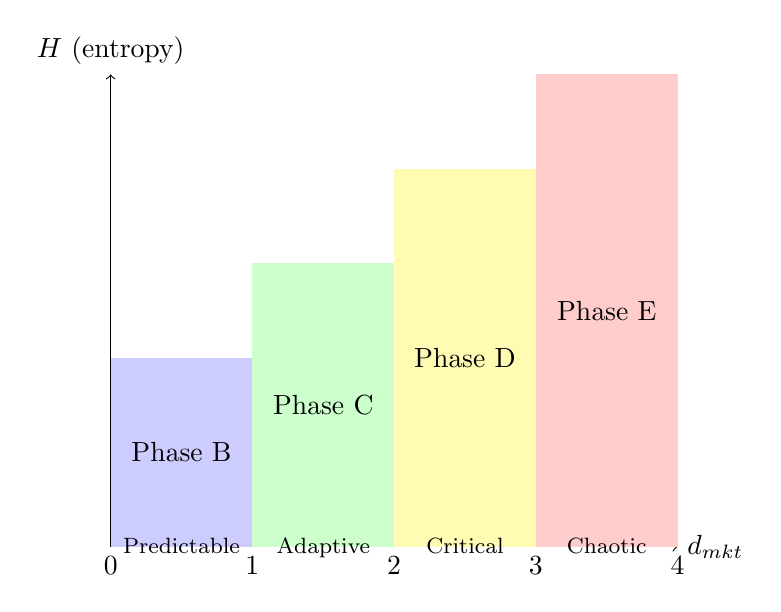
\begin{tikzpicture}[scale=1.2]
    % Axes
    \draw[->] (0,0) -- (6,0) node[right] {$d_{\text{mkt}}$};
    \draw[->] (0,0) -- (0,5) node[above] {$H$ (entropy)};
    
    % Regions
    \fill[blue!20] (0,0) rectangle (1.5,2);
    \node at (0.75,1) {Phase B};
    \node[below] at (0.75,0.2) {\footnotesize Predictable};
    
    \fill[green!20] (1.5,0) rectangle (3,3);
    \node at (2.25,1.5) {Phase C};
    \node[below] at (2.25,0.2) {\footnotesize Adaptive};
    
    \fill[yellow!30] (3,0) rectangle (4.5,4);
    \node at (3.75,2) {Phase D};
    \node[below] at (3.75,0.2) {\footnotesize Critical};
    
    \fill[red!20] (4.5,0) rectangle (6,5);
    \node at (5.25,2.5) {Phase E};
    \node[below] at (5.25,0.2) {\footnotesize Chaotic};
    
    % Labels
    \node[below] at (0,0) {0};
    \node[below] at (1.5,0) {1};
    \node[below] at (3,0) {2};
    \node[below] at (4.5,0) {3};
    \node[below] at (6,0) {4};
\end{tikzpicture}
\caption{Symbolic phase diagram of financial markets showing relationship between self-computing depth and entropy}
\label{fig:market_phase_diagram}
\end{figure}

This framework provides the complete theoretical foundation for understanding how Natural Observation-Based Computing applies not just to TSP, but to any system that can be viewed as a self-computing functorial object --- including financial markets, biological systems, and other naturally occurring computational processes.
